\documentclass[12pt,a4paper]{article}

\usepackage[utf8]{inputenc}
\usepackage[T1]{fontenc}
\usepackage{amsmath}
\usepackage{amsfonts}
\usepackage{amssymb}
\usepackage{graphicx}
% user details
\author{Athul}
\title{Introduction to LaTeX}

\begin{document}
	\maketitle
	\tableofcontents
	\newpage
	\section{Main Text}

	from Eq.\ref{eq1}
	
	TeXstudio is an integrated writing environment for creating LaTeX documents. Our goal is to make writing LaTeX as easy and comfortable as possible. Therefore TeXstudio has numerous features like syntax-highlighting, integrated viewer, reference checking, and various assistants. For more details see the features.
	
	TeXstudio is open-source and is available for all major operating systems.
	
	\textbf{Hello} \textit{How are you}
	
	\subsection{Sub Text}
	
	TeXstudio is an integrated writing environment for creating LaTeX documents. Our goal is to make writing LaTeX as easy and comfortable as possible. Therefore TeXstudio has numerous features like syntax-highlighting, integrated viewer, reference checking, and various assistants. For more details see the features.
	
$\partial$ \& \% text
	
	Let the wavelegth be, $\lambda$
	\section{Main Text 2}
	
	\begin{equation}
		y = \frac{x}{a}
	\end{equation}
\begin{equation}  \label{eq1}
	E = mc^2 
\end{equation}
	
	
	\begin{figure}[!b]
		\centering
		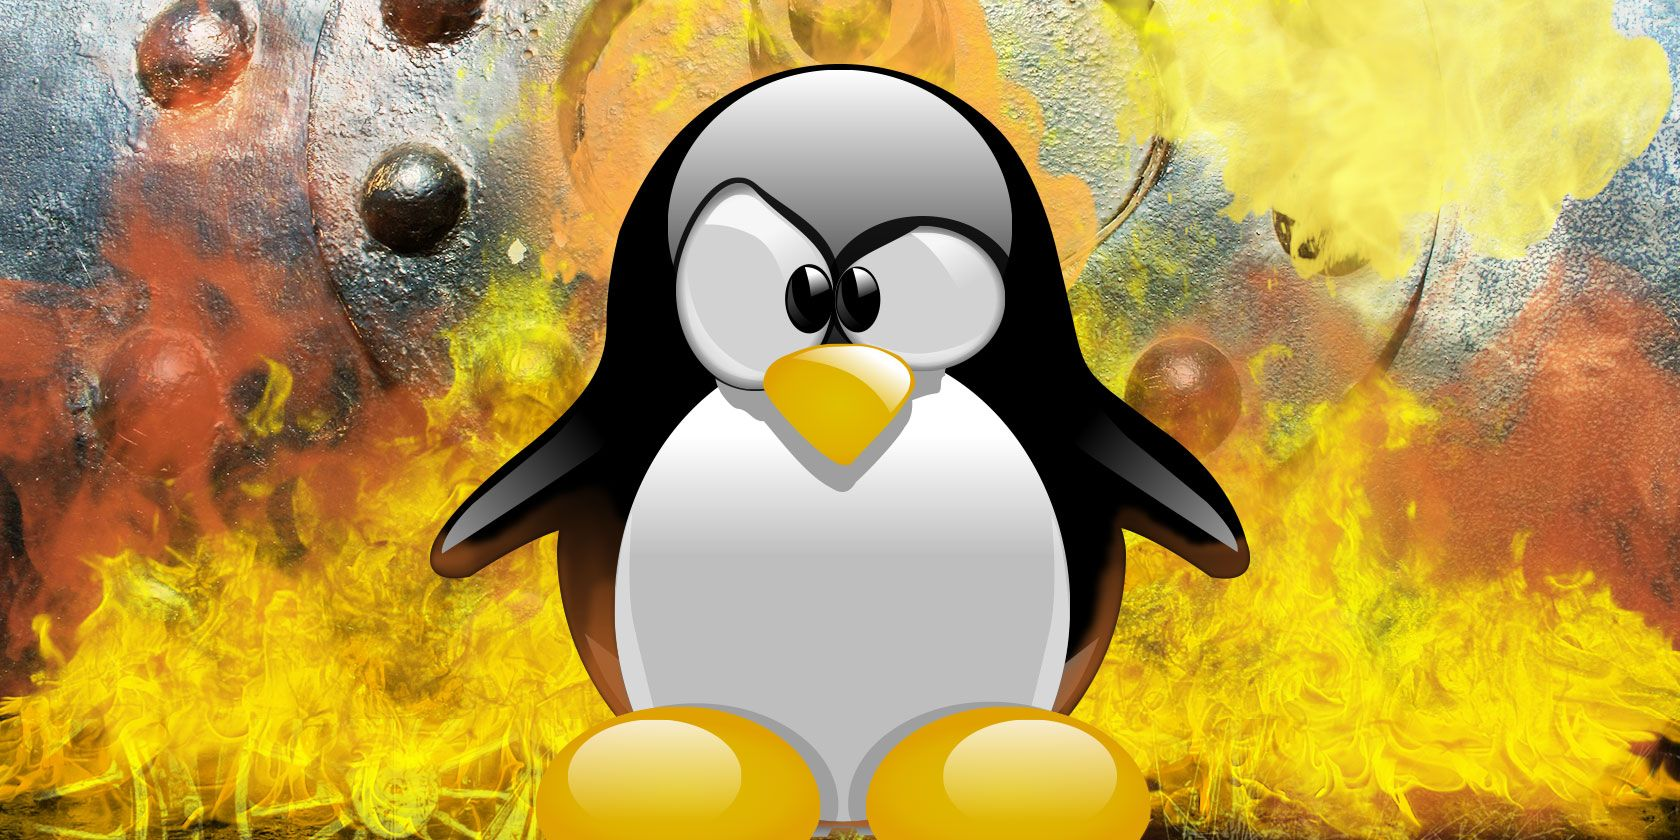
\includegraphics[width=0.8\textwidth]{linux.jpg}
	\end{figure}
\end{document}